% This file was created with tikzplotlib v0.10.1.
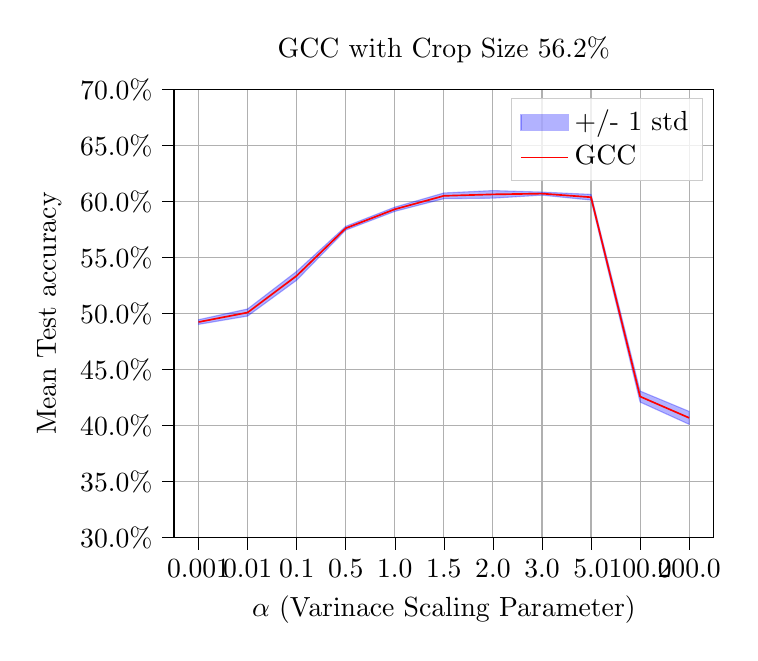
\begin{tikzpicture}

\definecolor{darkgray176}{RGB}{176,176,176}
\definecolor{lightgray204}{RGB}{204,204,204}

\begin{axis}[
legend cell align={left},
legend style={fill opacity=0.8, draw opacity=1, text opacity=1, draw=lightgray204},
tick align=outside,
tick pos=left,
title={GCC with Crop Size 56.2\%},
x grid style={darkgray176},
xlabel={\(\displaystyle \alpha\) (Varinace Scaling Parameter)},
xmajorgrids,
xmin=-0.5, xmax=10.5,
xtick style={color=black},
xtick={0,1,2,3,4,5,6,7,8,9,10},
xtick={0,1,2,3,4,5,6,7,8,9,10},
xticklabels={0.001,0.01,0.1,0.5,1.0,1.5,2.0,3.0,5.0,100.0,200.0},
xticklabels={0.001,0.01,0.1,0.5,1.0,1.5,2.0,3.0,5.0,100.0,200.0},
y grid style={darkgray176},
ylabel={Mean Test accuracy},
ymajorgrids,
ymin=0.3, ymax=0.7,
ytick style={color=black},
ytick={0.3,0.35,0.4,0.45,0.5,0.55,0.6,0.65,0.7},
yticklabels={30.0\%,35.0\%,40.0\%,45.0\%,50.0\%,55.0\%,60.0\%,65.0\%,70.0\%}
]
\path [draw=blue, fill=blue, opacity=0.3]
(axis cs:0,0.49455)
--(axis cs:0,0.49035)
--(axis cs:1,0.497772474757509)
--(axis cs:2,0.529771625913645)
--(axis cs:3,0.574471707216644)
--(axis cs:4,0.591187541391182)
--(axis cs:5,0.602490703221586)
--(axis cs:6,0.602969171699125)
--(axis cs:7,0.605660265593604)
--(axis cs:8,0.601253106467348)
--(axis cs:9,0.421068966299885)
--(axis cs:10,0.401177363398469)
--(axis cs:10,0.412722636601531)
--(axis cs:10,0.412722636601531)
--(axis cs:9,0.430881033700115)
--(axis cs:8,0.606346893532652)
--(axis cs:7,0.608389734406396)
--(axis cs:6,0.609730828300875)
--(axis cs:5,0.607609296778414)
--(axis cs:4,0.594962458608818)
--(axis cs:3,0.577828292783357)
--(axis cs:2,0.537678374086355)
--(axis cs:1,0.504127525242491)
--(axis cs:0,0.49455)
--cycle;
\addlegendimage{area legend, draw=blue, fill=blue, opacity=0.3}
\addlegendentry{+/- 1 std}

\addplot [semithick, red, opacity=1]
table {%
0 0.49245
1 0.50095
2 0.533725
3 0.57615
4 0.593075
5 0.60505
6 0.60635
7 0.607025
8 0.6038
9 0.425975
10 0.40695
};
\addlegendentry{GCC}
\end{axis}

\end{tikzpicture}
